% note.tex — φ^3 理論：模型の定義と1ループの構造（d = 4, 6）
% コンパイル: lualatex note.tex（参照解決のため2回）
\documentclass[a4paper,10pt]{ltjsarticle}
\usepackage[margin=20mm]{geometry}
\usepackage[haranoaji,deluxe]{luatexja-preset}
\ltjsetparameter{jacharrange={-3}}
\usepackage{amsmath,amssymb}
\usepackage{booktabs,tabularx,array}
\usepackage[table]{xcolor}
\usepackage{tikz}
\usetikzlibrary{arrows.meta,calc,positioning}
\usepackage[font=small,labelfont=bf]{caption}
\usepackage{graphicx}
\usepackage{xurl}
\usepackage{hyperref}
\hypersetup{colorlinks=true,linkcolor=blue!50!black,citecolor=green!40!black,urlcolor=blue!60!black,
  pdftitle={phi^3 theory: model and one-loop structure},pdfauthor={}}

\definecolor{divc}{RGB}{190,30,30}
\definecolor{finc}{RGB}{52,128,72}
\renewcommand{\jsParagraphMark}{\textcolor{black!65}{\rule[-0.02\zw]{0.62\zw}{0.62\zw}}\hspace{0.35\zw}}
\newcommand{\dd}{\mathrm{d}}
\newcommand{\Kfour}{(4\pi)^2}
\newcommand{\Ksix}{(4\pi)^3}

\tikzset{
  prop/.style={thick},
  vtx/.style={circle,fill=black,inner sep=1.3pt},
  ctv/.style={circle,draw=black,fill=white,inner sep=0pt,minimum size=7pt,path picture={
      \draw (path picture bounding box.north west) -- (path picture bounding box.south east)
            (path picture bounding box.south west) -- (path picture bounding box.north east);}},
  mom/.style={-{Stealth[length=1.6mm]},thin},
  lab/.style={font=\small,align=center},
}

\title{$\phi^3$ 理論：模型の定義と1ループの構造（$d=4,\,6$）}
\author{}
\date{2026年10月9日}

\begin{document}
\maketitle

\begin{abstract}
新しく組んだループ計算環境（FeynCalc、Package-X、LoopTools、FeynRules、MadGraph）を練習し検算するための玩具模型として、質量 $m$ を持つ実スカラー1つの $\phi^3$ 理論を定義し、時空次元 $d=4$ と $d=6$ の両方で扱う。ラグランジアンから Feynman 則と対称性因子を導き、べき数え上げと Feynman パラメータ表示によって、1ループのタドポール・自己エネルギー・頂点補正の紫外発散を両方の次元で求めた。$d=4$ では発散するのはタドポールと、自己エネルギーのうち外運動量によらない部分だけで、最小引き算の対抗項は質量項 $\delta_m=g^2/(2(4\pi)^2\epsilon)$ だけが残る（$\delta_Z=\delta_g=0$）。$d=6$ では三つとも発散し、$\delta_Z=-g^2/(12(4\pi)^3\epsilon)$、$\delta_m=-g^2m^2/(2(4\pi)^3\epsilon)$、$\delta_g=-g^3/(2(4\pi)^3\epsilon)$ となる。ここから $\beta(g)=-3g^3/(4(4\pi)^3)$ が出て、理論は漸近自由である。$d=4$ では結合定数は1ループで走らず、質量は $\mu\,\dd m^2/\dd\mu=g^2/(4\pi)^2$ で走る。最後に、これらの手計算を各ツールの出力と突き合わせる計画を定め（比べる量、方法、一致の基準、数値の基準点 $m=g=\mu=1$）、その最初の三段階を実行した。FeynRules の模型ファイルから書き出した FeynArts 模型で作った木の振幅は、式と記号として一致した。MadGraph の断面積は、$\sqrt{s}=2.5,\,5,\,10$ で式の数値積分と統計誤差の1.3倍以内で一致した。$d=4$ の1ループでは、FeynCalc の振幅、発散部分、対抗項が手計算と記号として一致した。有限部分 $B_0$ は Package-X・LoopTools・COLLIER の三つとも閉じた式と相対 $4\times10^{-15}$ 以内で一致し、虚部は光学定理 $\mathrm{Im}\,B_0=\pi\beta$ を満たした。一方、この環境の LoopTools は閾値より下の $C_0$ を誤って返すことが分かった。導出はすべて付録に省略なく載せる。
\end{abstract}

\section{目的と問い}\label{sec:intro}

本ノートの問いは次の一つである。\textbf{$\phi^3$ 理論の1ループの紫外発散と繰り込みの構造は、$d=4$ と $d=6$ でどう違うか。そして、どの量をどの手段で突き合わせれば、計算環境の各部品を独立に検算できるか。}この問いを立てる理由は、ループ計算の環境を組み直したばかりで、その各部品がこちらの意図どおりに動くことを、手計算で答えが分かる模型で確かめたいからである~\cite{env}。$\phi^3$ 理論は3点結合を持つ最も簡単な相互作用理論であり、1ループの量はすべて手で計算できる。しかも次元によって性格が大きく変わる。$d=4$ では結合定数が質量次元を持つ超繰り込み可能な理論で、Package-X と LoopTools がそのまま使える。$d=6$ では繰り込み可能で漸近自由な理論になり、場・質量・結合のすべてが繰り込まれる~\cite{srednicki}。$d=6$ の積分は Package-X と LoopTools の守備範囲（$D=4-2\epsilon$）の外にあるので、FeynCalc を $D\neq4$ で使う練習にもなる。

求める量は四つである。(i) Feynman 則と対称性因子。(ii) 1ループのスカラー積分 $I_1,I_2,I_3$ の紫外発散部分。(iii) 最小引き算（MS）の1ループ対抗項と、繰り込み群の係数（$d=6$ の $\beta$ 関数、$d=4$ の質量の走り）。(iv) 木レベルの $\phi\phi\to\phi\phi$ 振幅。手計算とツールの間で求める一致は、発散部分と対抗項では記号として完全な一致、有限部分では数値基準点での倍精度の一致である。

本ノートの構成は次の通りである。第~\ref{sec:setup} 節で模型と前提を定める。第~\ref{sec:results} 節で上の (i)〜(iv) の結果を述べる。第~\ref{sec:plan} 節で、これらを各ツールと突き合わせる計画を定める。第~\ref{sec:checks} 節で、その手順 (1)〜(3) の結果を示す。第~\ref{sec:discussion} 節で未決の点と今後の手順をまとめる。導出は\ref{app:rules}〜\ref{app:b0} にある。

\section{設定}\label{sec:setup}

模型は、質量 $m$ を持つ実スカラー場 $\phi$ が1つだけあり、3次の自己相互作用を持つ理論である。ラグランジアン密度は
\begin{equation}
\mathcal{L}=\frac12\,\partial_\mu\phi\,\partial^\mu\phi-\frac12 m^2\phi^2-\frac{g\mu^{\epsilon}}{3!}\,\phi^3+Y\phi
+\frac12\,\delta_Z\,\partial_\mu\phi\,\partial^\mu\phi-\frac12\,\delta_m\phi^2-\frac{\delta_g\mu^{\epsilon}}{3!}\,\phi^3
\label{eq:L}
\end{equation}
とする。最初の4項が繰り込まれた量で書いた模型、残り3項が対抗項である。線形項 $Y\phi$ は、ループが作る1点関数（タドポール）を各次数でちょうど打ち消し、$\langle\phi\rangle=0$ を保つために置く。以前に作った FeynRules の模型ファイル（\nolinkurl{models/backup_20261009/feynrules_Library_Models/Phi3/Phi3.fr}）は $\mathcal{L}\supset-(\lambda/6)\phi^3$ と書いていたが、これは本ノートの $g$ と同じもの（$\lambda\equiv g$）である。$\phi^4$ の結合定数と区別するため、本ノートでは $g$ と書く。

\paragraph{前提。}本ノートは次の前提に立つ。
\begin{enumerate}
\item 計量は $(+,-,-,-)$、$\hbar=c=1$ とする。
\item 場は質量 $m$ の実スカラー1つで、相互作用は $\phi^3$ だけとする。$\phi^4$ などの他の相互作用は入れない。
\item 時空次元は $d=4$ と $d=6$ の二つを扱う。ループ積分は次元正則化で行い、$D=d-2\epsilon$ とする。$\phi$ の質量次元は $(D-2)/2$、$g$ の質量次元は $3-d/2$ なので、どちらの次元でも結合定数を $g\mu^{\epsilon}$ と書く（\ref{app:counting}）。
\item 紫外発散は最小引き算（MS）で処理する。すなわち、対抗項は $1/\epsilon$ の極だけを打ち消す。有限部分の規約（$\overline{\mathrm{MS}}$ にするか on-shell にするか）は、有限部分を計算する段階で決める。
\item タドポールは $Y$ で各次数ちょうど打ち消す。そのため、外線にタドポールが付いた図は計算に含めない。FeynArts では \texttt{ExcludeTopologies -> Tadpoles} に当たる。
\item $\phi^3$ のポテンシャルは下に有界でない。本模型は摂動論の範囲でだけ扱う玩具模型である。
\item 数値を比べるときの基準点は $m=1$、$g=1$、$\mu=m$ とする（$d=4$ では $g$ は $m$ を単位とする）。
\end{enumerate}
本文で使う記号を表~\ref{tab:notation} にまとめる。

\begin{table}[tbp]
\centering\small
\caption{本ノートで使う記号。}
\label{tab:notation}
\begin{tabularx}{\linewidth}{>{\raggedright\arraybackslash}p{3.3cm}X}
\toprule
\textbf{記号} & \textbf{意味} \\
\midrule
$\phi$, $m$ & 実スカラー場と、その（繰り込まれた）質量 \\
$g$ & 3点結合定数（旧模型ファイルの $\lambda$、模型ファイル \texttt{Src/Phi3.fr} の \texttt{gphi} と同じ）。$d=4$ では質量次元1、$d=6$ では無次元 \\
$Y$ & 線形項の係数。タドポールを打ち消すように決める \\
$d$, $D$, $\epsilon$ & 時空次元（4 または 6）、正則化した次元 $D=d-2\epsilon$、その差 \\
$\mu$ & 繰り込みスケール。結合定数の次元を補う因子 $\mu^\epsilon$ に現れる \\
$\delta_Z,\ \delta_m,\ \delta_g$ & 場・質量・結合の対抗項。$Z\equiv1+\delta_Z$ \\
$I_N$ & $N$ 本の伝播関数を持つ1ループのスカラー積分 \\
$x_j$, $\Delta$ & Feynman パラメータと、それで束ねた分母の定数部分（\ref{app:integrals}） \\
$V_n$ & 1PI の $n$ 点関数。Feynman 則のとおり、$i$ の因子を含めた図の和 \\
$s,\ t,\ u$ & Mandelstam 変数。$s+t+u=4m^2$ \\
$\beta(g)$ & $\beta\equiv\dd g/\dd\ln\mu$（$\epsilon\to0$ の値） \\
$E,\ V,\ L,\ I$ & 図の外線、頂点、ループ、内線の数 \\
\bottomrule
\end{tabularx}
\end{table}

\section{結果}\label{sec:results}

\paragraph{Feynman 則と対称性因子。}式~\eqref{eq:L} から読み取れる Feynman 則を図~\ref{fig:rules} に示す。伝播関数は $i/(p^2-m^2+i0)$、3点頂点は $-ig\mu^\epsilon$、線形項は $iY$ である。対抗項は、2点の挿入 $i(\delta_Zp^2-\delta_m)$ と3点の挿入 $-i\delta_g\mu^\epsilon$ になる。1ループの1PI 図は図~\ref{fig:oneloop} の3つで、対称性因子はタドポールと自己エネルギーが $1/2$、頂点補正の三角形が $1$ である。いずれも Wick の縮約を数えて導いた（\ref{app:rules}）。旧模型ファイルを FeynArts 用に書き出したものでも、頂点は \texttt{C[S[1],S[1],S[1]] == -I lam} になっていて、上の $-ig$ と一致する。

\begin{figure}[tbp]
\centering
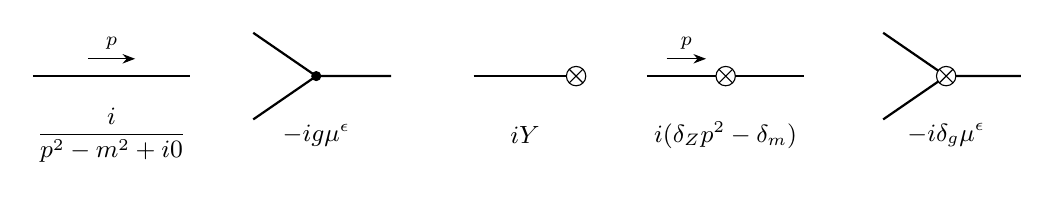
\begin{tikzpicture}
% propagator
\begin{scope}[shift={(0,0)}]
  \draw[prop] (0,0) -- (2,0);
  \draw[mom] (0.7,0.22) -- (1.3,0.22) node[midway,above,font=\scriptsize] {$p$};
  \node[lab] at (1,-0.75) {$\dfrac{i}{p^2-m^2+i0}$};
\end{scope}
% vertex
\begin{scope}[shift={(3.6,0)}]
  \draw[prop] (0,0) -- (-0.8,0.55) (0,0) -- (-0.8,-0.55) (0,0) -- (0.95,0);
  \node[vtx] at (0,0) {};
  \node[lab] at (0,-0.75) {$-ig\mu^{\epsilon}$};
\end{scope}
% linear term
\begin{scope}[shift={(5.6,0)}]
  \draw[prop] (0,0) -- (1.3,0);
  \node[ctv] at (1.3,0) {};
  \node[lab] at (0.65,-0.75) {$iY$};
\end{scope}
% 2-point counterterm
\begin{scope}[shift={(7.8,0)}]
  \draw[prop] (0,0) -- (2,0);
  \node[ctv] at (1,0) {};
  \draw[mom] (0.25,0.22) -- (0.75,0.22) node[midway,above,font=\scriptsize] {$p$};
  \node[lab] at (1,-0.75) {$i(\delta_Zp^2-\delta_m)$};
\end{scope}
% 3-point counterterm
\begin{scope}[shift={(11.6,0)}]
  \draw[prop] (0,0) -- (-0.8,0.55) (0,0) -- (-0.8,-0.55) (0,0) -- (0.95,0);
  \node[ctv] at (0,0) {};
  \node[lab] at (0,-0.75) {$-i\delta_g\mu^{\epsilon}$};
\end{scope}
\end{tikzpicture}
\caption{式~\eqref{eq:L} から導いた Feynman 則（\ref{app:rules}）。左から伝播関数、3点頂点、線形項、2点の対抗項、3点の対抗項。$\otimes$ は対抗項（と線形項）の挿入を表す。ループ運動量 $k$ ごとに $\int\dd^Dk/(2\pi)^D$ を掛け、対称性因子で割る。}
\label{fig:rules}
\end{figure}

\paragraph{べき数え上げ。}外線 $E$ 本、頂点 $V$ 個の図の表面的な発散次数は
\begin{equation}
\omega=d-\frac{d-2}{2}\,E+\frac{d-6}{2}\,V
\label{eq:omega}
\end{equation}
である（\ref{app:counting}）。$d=4$ では $\omega=4-E-V$ となり、頂点が増えるほど収束がよくなる。発散する図は有限個に限られ、理論は超繰り込み可能である。$d=6$ では $\omega=6-2E$ で $V$ によらず、$E\le3$ の関数がすべての次数で発散する。これは繰り込み可能な理論の振る舞いである。1ループの1PI 図では $E=V$ なので、どちらの次元でも $\omega=d-2E$ となる。

\begin{figure}[tbp]
\centering
\begin{tikzpicture}
% tadpole
\begin{scope}[shift={(0,0)}]
  \draw[prop] (-1.2,0) -- (0,0);
  \draw[prop] (0,0.55) circle (0.55);
  \node[vtx] at (0,0) {};
  \node[lab] at (0,-0.6) {タドポール $V_1$};
  \node[lab,font=\footnotesize] at (0,-1.1) {対称性因子 $1/2$};
\end{scope}
% self-energy
\begin{scope}[shift={(5.0,0)}]
  \draw[prop] (-1.6,0) -- (-0.6,0) (0.6,0) -- (1.6,0);
  \draw[prop] (0,0) circle (0.6);
  \node[vtx] at (-0.6,0) {}; \node[vtx] at (0.6,0) {};
  \draw[mom] (-1.45,0.2) -- (-0.95,0.2) node[midway,above,font=\scriptsize] {$p$};
  \node[lab] at (0,-0.95) {自己エネルギー $V_2$};
  \node[lab,font=\footnotesize] at (0,-1.45) {対称性因子 $1/2$};
\end{scope}
% triangle
\begin{scope}[shift={(10.2,0)}]
  \coordinate (A) at (-0.65,0); \coordinate (B) at (0.45,0.65); \coordinate (C) at (0.45,-0.65);
  \draw[prop] (A) -- (B) -- (C) -- cycle;
  \draw[prop] (A) -- (-1.4,0) (B) -- (1.05,1.1) (C) -- (1.05,-1.1);
  \node[vtx] at (A) {}; \node[vtx] at (B) {}; \node[vtx] at (C) {};
  \node[lab] at (0,-1.45) {頂点補正 $V_3$};
  \node[lab,font=\footnotesize] at (0,-1.95) {対称性因子 $1$};
\end{scope}
\end{tikzpicture}
\caption{1ループの1PI 図と、その対称性因子（\ref{app:rules}）。外線にタドポールが付いた図は線形項 $Y$ で打ち消すので含めない。}
\label{fig:oneloop}
\end{figure}

\paragraph{1ループ積分の発散部分。}1ループのスカラー積分を
\begin{equation}
I_N(q_1,\dots,q_N)\equiv\int\frac{\dd^Dk}{(2\pi)^D}\prod_{j=1}^{N}\frac{1}{(k+q_j)^2-m^2+i0}
\label{eq:IN}
\end{equation}
と定義する。Feynman パラメータでまとめ、Wick 回転して積分すると、$N$ と $d$ によらない次の一般式が得られる（\ref{app:integrals}）。
\begin{equation}
I_N=\frac{i(-1)^N\,\Gamma(N-D/2)}{(4\pi)^{D/2}}\int\!\dd F\,\Delta^{D/2-N},\qquad
\Delta=m^2-\sum_j x_jq_j^2+\Bigl(\sum_j x_jq_j\Bigr)^2 .
\label{eq:IN-general}
\end{equation}
発散は $\Gamma(N-D/2)$ の極からだけ生じ、$k\equiv d/2-N$ が0以上の整数のとき現れる。その極の部分は
\begin{equation}
I_N\Big|_{\text{pole}}=\frac{i\,(-1)^{N+k}}{(4\pi)^{d/2}\,k!\,\epsilon}\int\!\dd F\,\Delta^{k}
\label{eq:poleN}
\end{equation}
である。$k<0$ なら $I_N$ は有限である。これを $N=1,2,3$ に当てはめた結果を、表面的な発散次数とあわせて表~\ref{tab:poles} に示す。$d=4$ では $I_2$ の極が外運動量によらず、$I_3$ は有限である。$d=6$ では三つとも発散し、$I_2$ の極は $p^2$ に依存する。この違いが、次に述べる繰り込みの構造の違いを生む。

\begin{table}[tbp]
\centering\small
\caption{1ループのスカラー積分の表面的な発散次数 $\omega=d-2N$（式~\eqref{eq:omega}）と紫外発散部分（式~\eqref{eq:poleN}）。$I_1$ は質量 $m$ のタドポール積分、$I_2$ は外運動量 $p$ の2点積分（$q_1=0$、$q_2=p$）、$I_3$ は3点積分である。}
\label{tab:poles}
\begin{tabular}{lcccc}
\toprule
& \multicolumn{2}{c}{$d=4$} & \multicolumn{2}{c}{$d=6$} \\
\cmidrule(lr){2-3}\cmidrule(lr){4-5}
& $\omega$ & 発散部分 & $\omega$ & 発散部分 \\
\midrule
$I_1$ & $2$ & $\dfrac{i\,m^2}{(4\pi)^2\epsilon}$ & $4$ & $-\dfrac{i\,m^4}{2(4\pi)^3\epsilon}$ \\[2ex]
$I_2(p^2)$ & $0$ & $\dfrac{i}{(4\pi)^2\epsilon}$ & $2$ & $-\dfrac{i}{(4\pi)^3\epsilon}\Bigl(m^2-\dfrac{p^2}{6}\Bigr)$ \\[2ex]
$I_3$ & $-2$ & 有限 & $0$ & $-\dfrac{i}{2(4\pi)^3\epsilon}$ \\
\bottomrule
\end{tabular}
\end{table}

\paragraph{1ループの1PI 関数。}図~\ref{fig:oneloop} の図を Feynman 則で書き、対抗項を加えると、1PI の1点・2点・3点関数は
\begin{equation}
V_1=iY+\frac{g\mu^\epsilon}{2}\,I_1,\qquad
V_2(p^2)=\frac{g^2\mu^{2\epsilon}}{2}\,I_2(p^2)+i\bigl(\delta_Zp^2-\delta_m\bigr),\qquad
V_3=g^3\mu^{3\epsilon}\,I_3-i\,\delta_g\mu^{\epsilon}
\label{eq:V}
\end{equation}
となる（\ref{app:ren}）。タドポールの条件 $V_1=0$ から $Y=(ig\mu^\epsilon/2)\,I_1$ と決まる。$I_1$ は純虚数なので、$Y$ は実数である。

\paragraph{最小引き算の対抗項。}$V_2$ と $V_3$ の $1/\epsilon$ の極が消えるように対抗項を決める（\ref{app:ren}）。$d=4$ では、自己エネルギーの極が外運動量によらず、頂点補正は有限なので、
\begin{equation}
d=4:\qquad \delta_Z=0,\qquad \delta_m=\frac{g^2}{2(4\pi)^2\epsilon},\qquad \delta_g=0 .
\label{eq:ct4}
\end{equation}
$d=6$ では三つとも必要で、
\begin{equation}
d=6:\qquad \delta_Z=-\frac{g^2}{12(4\pi)^3\epsilon},\qquad \delta_m=-\frac{g^2m^2}{2(4\pi)^3\epsilon},\qquad \delta_g=-\frac{g^3}{2(4\pi)^3\epsilon}.
\label{eq:ct6}
\end{equation}
Srednicki は $d=6-\epsilon_{\mathrm S}$ と書くので、$1/\epsilon_{\mathrm S}=1/(2\epsilon)$ である。$\alpha\equiv g^2/(4\pi)^3$ と置くと、式~\eqref{eq:ct6} は $Z_\phi=1-\alpha/(6\epsilon_{\mathrm S})$、$Z_m=1-\alpha/\epsilon_{\mathrm S}$、$Z_g=1-\alpha/\epsilon_{\mathrm S}$ と書き直せる。これは同書の値と一致する~\cite{srednicki}。

\paragraph{繰り込み群。}裸の量が $\mu$ によらないことから、繰り込まれた量の走り方が決まる（\ref{app:ren}）。$d=6$ では
\begin{equation}
\beta(g)=-\frac{3g^3}{4(4\pi)^3}
\label{eq:beta6}
\end{equation}
となり、結合定数は高エネルギーで小さくなる（漸近自由）。$d=4$ では、1ループで $\delta_Z=\delta_g=0$ なので、結合定数は（次元の分 $-\epsilon g$ を除いて）走らない。一方、質量は
\begin{equation}
d=4:\qquad \mu\frac{\dd m^2}{\dd\mu}=\frac{g^2}{(4\pi)^2}
\label{eq:mrun4}
\end{equation}
で走る。$g$ が質量次元を持つので、$m^2$ の走りは $m$ によらない加法的なものになる。

\paragraph{木レベルの散乱振幅。}$\phi\phi\to\phi\phi$ の木の振幅は、$s,t,u$ の3つのチャンネルの和
\begin{equation}
\mathcal{M}=-g^2\left[\frac{1}{s-m^2}+\frac{1}{t-m^2}+\frac{1}{u-m^2}\right]
\label{eq:Mtree}
\end{equation}
である（図~\ref{fig:tree}、\ref{app:tree}）。各チャンネルの対称性因子は1である。

\begin{figure}[tbp]
\centering
\begin{tikzpicture}
\begin{scope}[shift={(0,0)}]
  \draw[prop] (-1.2,0.7) -- (-0.5,0) -- (-1.2,-0.7) (-0.5,0) -- (0.5,0) (1.2,0.7) -- (0.5,0) -- (1.2,-0.7);
  \node[vtx] at (-0.5,0) {}; \node[vtx] at (0.5,0) {};
  \node[font=\scriptsize] at (-1.4,0.8) {1}; \node[font=\scriptsize] at (-1.4,-0.8) {2};
  \node[font=\scriptsize] at (1.4,0.8) {3}; \node[font=\scriptsize] at (1.4,-0.8) {4};
  \node[lab] at (0,-1.65) {$s$ チャンネル：$\dfrac{-ig^2}{s-m^2}$};
\end{scope}
\begin{scope}[shift={(4.8,0)}]
  \draw[prop] (-1.0,0.9) -- (0,0.45) -- (1.0,0.9) (0,0.45) -- (0,-0.45) (-1.0,-0.9) -- (0,-0.45) -- (1.0,-0.9);
  \node[vtx] at (0,0.45) {}; \node[vtx] at (0,-0.45) {};
  \node[font=\scriptsize] at (-1.2,1.0) {1}; \node[font=\scriptsize] at (1.2,1.0) {3};
  \node[font=\scriptsize] at (-1.2,-1.0) {2}; \node[font=\scriptsize] at (1.2,-1.0) {4};
  \node[lab] at (0,-1.75) {$t$ チャンネル：$\dfrac{-ig^2}{t-m^2}$};
\end{scope}
\begin{scope}[shift={(9.6,0)}]
  \draw[prop] (-1.0,0.9) -- (0,0.45) (0,0.45) -- (1.0,-0.9) (0,0.45) -- (0,-0.45) (-1.0,-0.9) -- (0,-0.45) (0,-0.45) -- (1.0,0.9);
  \node[vtx] at (0,0.45) {}; \node[vtx] at (0,-0.45) {};
  \node[font=\scriptsize] at (-1.2,1.0) {1}; \node[font=\scriptsize] at (1.2,1.0) {3};
  \node[font=\scriptsize] at (-1.2,-1.0) {2}; \node[font=\scriptsize] at (1.2,-1.0) {4};
  \node[lab] at (0,-1.75) {$u$ チャンネル：$\dfrac{-ig^2}{u-m^2}$};
\end{scope}
\end{tikzpicture}
\caption{$\phi(p_1)\phi(p_2)\to\phi(p_3)\phi(p_4)$ の木の図。$s=(p_1+p_2)^2$、$t=(p_1-p_3)^2$、$u=(p_1-p_4)^2$。三つの和が $i\mathcal{M}$（式~\eqref{eq:Mtree}）を与える。}
\label{fig:tree}
\end{figure}

\section{検算の計画}\label{sec:plan}

第~\ref{sec:results} 節の各量を、どの手段で計算して突き合わせるかを表~\ref{tab:plan} に示す。手計算（付録）を基準とし、ツールの出力がそれと一致するかを確かめる。使うツールの版と配置は、計算環境の記録~\cite{env} にある。FeynCalc 10.2.1 と FeynHelpers 2、Package-X 2.1.1、LoopTools 2.16、FeynRules 2.3.49、\texttt{MG5\_aMC@NLO} 3.8.1 である。

\begin{table}[tbp]
\centering\small
\caption{各量と、それを計算して突き合わせる手段。「—」はその手段を使わないことを表す。}
\label{tab:plan}
\begin{tabularx}{\linewidth}{>{\raggedright\arraybackslash}p{3.2cm}>{\raggedright\arraybackslash}p{2.0cm}>{\raggedright\arraybackslash}X>{\raggedright\arraybackslash}p{2.0cm}>{\raggedright\arraybackslash}p{1.7cm}>{\raggedright\arraybackslash}p{1.9cm}}
\toprule
\textbf{量} & \textbf{手計算} & \textbf{FeynCalc（+ FeynArts）} & \textbf{Package-X} & \textbf{LoopTools} & \textbf{MadGraph} \\
\midrule
Feynman 則・対称性因子 & \ref{app:rules} & FeynRules から書き出した FeynArts 模型の係数と、生成した図の対称性因子 & — & — & UFO の頂点 \\
木の振幅 \eqref{eq:Mtree} & \ref{app:tree} & 記号として一致 & — & — & $d=4$ の断面積 \\
$d=4$：$I_N$ の極、対抗項 \eqref{eq:ct4} & \ref{app:integrals}, \ref{app:ren} & TID で PaVe 関数へ、極を抽出 & 解析式 & — & — \\
$d=4$：有限部分 & Feynman パラメータ積分の数値 & — & 解析式 & 数値 & — \\
$d=6$：$I_N$ の極、対抗項 \eqref{eq:ct6}、$\beta$ \eqref{eq:beta6} & \ref{app:integrals}, \ref{app:ren} & $D=6-2\epsilon$ で計算 & 使えない & 使えない & — \\
$d=6$：有限部分 & Feynman パラメータ積分の数値 & — & 使えない & 使えない & — \\
\bottomrule
\end{tabularx}
\end{table}

\paragraph{一致の基準。}発散部分と対抗項は、$1/\epsilon$ の係数が記号として完全に一致することを求める。有限部分は、基準点 $m=g=\mu=1$ で、Package-X の解析式・LoopTools の数値・Feynman パラメータ積分の数値積分が、倍精度の丸め誤差の範囲（相対 $10^{-12}$ 程度）で一致することを求める。有限部分は規約に依存するので、比べる前にツールごとの規格化をそろえる。計算環境の記録で確かめたとおり、FeynCalc を通した $B_0$ は、LoopTools の規格化と $-(\gamma_E+\ln\pi)$ だけずれている~\cite{env}。MadGraph の断面積は、式~\eqref{eq:Mtree} を自分で数値積分した値と、統計誤差の範囲で一致することを求める。

\paragraph{手順。}次の順に進める。(1) 模型ファイル \texttt{Phi3.fr} を \texttt{Src/} に作り、FeynRules で FeynArts の模型と UFO を書き出して、Feynman 則を確かめる。(2) 木の振幅を FeynCalc と MadGraph で確かめる。(3) $d=4$ の1ループ（極、対抗項、有限部分）を FeynCalc・Package-X・LoopTools で確かめる。(4) $d=6$ の1ループを FeynCalc で $D=6-2\epsilon$ として計算し、式~\eqref{eq:ct6} と式~\eqref{eq:beta6} を再現する。

\section{検算の結果}\label{sec:checks}

第~\ref{sec:plan} 節の手順のうち、(1) 模型ファイルの作成、(2) 木の振幅の検算、(3) $d=4$ の1ループの検算を行った。使ったスクリプトはすべて \texttt{Src/} にある。模型ファイルからの書き出しは \texttt{generate\_Phi3.wl} で、木の検算は \texttt{run\_tree\_check.sh} で、1ループの検算は \texttt{run\_oneloop4\_check.sh} で再実行できる。

\paragraph{手順 (1)：模型ファイル。}FeynRules の模型ファイル \texttt{Src/Phi3.fr} を作った。ラグランジアンは式~\eqref{eq:L} から対抗項と線形項を除いた部分である。結合定数 $g$ はパラメータ \texttt{gphi}（TeX 表記は $g$）と書いた。\texttt{g} という名前にすると、FeynRules 2.3.49 の UFO 出力が \texttt{\$RecursionLimit} に達して止まるためである。名前だけを変えた比較で、原因がこの名前であることを確かめた。FeynRules のチェック（エルミート性、運動項の規格化、質量スペクトル）はすべて通り、頂点は $-i\,\texttt{gphi}$ となって図~\ref{fig:rules} の $-ig$ と一致した。FeynArts 模型（\texttt{C[S[1],S[1],S[1]] == -I gphi}）と UFO も \texttt{Src/generated/} に書き出せた。MadGraph 3.8.1 はその UFO から $\phi\phi\to\phi\phi$ の図を $s,t,u$ の3つ生成した。なお、旧模型ファイルは運動項を \texttt{D[phi, mu]} と書いていた。これは Mathematica の記号 \texttt{mu} による微分なので 0 になり、旧ファイルのラグランジアンには運動項がなかった。実際に読み込んで評価すると、$-\frac12m^2\phi^2-\frac{\lambda}{6}\phi^3$ だけが残る。頂点は3次の項だけで決まるので、旧ファイルから書き出した FeynArts の頂点には影響しなかったと考えられる。新しいファイルでは FeynRules の偏微分 \texttt{del} を使っている。

\paragraph{手順 (2)：木の振幅。}\texttt{Src/generated/Phi3\_FA} の FeynArts 模型から $\phi\phi\to\phi\phi$ の木の図を作ると、$s,t,u$ の3つが対称性因子 $1$ で現れた。FeynCalc で振幅を組み立てて Mandelstam 変数で書くと、式~\eqref{eq:Mtree} との差は記号として $0$ になった。数値でも、$\sqrt{s}=5$、$\cos\theta=0.3$、$m=g=1$ で $\mathcal{M}=0.1463531980$ となり、式~\eqref{eq:Mtree} を Python で評価した値と一致した。FeynArts の \texttt{CreateFeynAmp} は既定で因子 $-i$ を掛けるので、出力は図の和 $i\mathcal{M}$ ではなく $\mathcal{M}$ そのものになる。FeynRules の模型には、一時フォルダに置いたコピーに FeynCalc 用のパッチ（\texttt{FAPatch}）を当ててから読み込んだ。

続いて、UFO を MadGraph 3.8.1 に読み込ませ、$\phi$ どうしを固定エネルギーで衝突させて全断面積を求めた。カットはかけず、$m=g=1$（単位は GeV）とした。比べる相手は、式~\eqref{eq:Mtree} の $|\mathcal{M}|^2$ を角度について数値積分した
\begin{equation}
\sigma=\frac12\int\!\dd\Omega\,\frac{|\mathcal{M}|^2}{64\pi^2s},\qquad
t=-2p^2(1-\cos\theta),\quad u=-2p^2(1+\cos\theta),\quad p^2=\frac{s}{4}-m^2
\label{eq:sigma}
\end{equation}
である（\ref{app:xsec}）。因子 $1/2$ は、終状態の二つの $\phi$ が同種粒子であることから来る。表~\ref{tab:tree} に示すように、$\sqrt{s}=2.5,\,5,\,10$ のすべてで、MadGraph の値は式~\eqref{eq:sigma} と統計誤差の1.3倍以内で一致した。なお、MadGraph は読み込んだ UFO に残る Python 2 の構文をその場で Python 3 に書き換える。そこで \texttt{Src/work/} に置いたコピーを読ませ、\texttt{Src/generated/} は FeynRules の出力のまま保った。

\begin{table}[tbp]
\centering\small
\caption{$\phi\phi\to\phi\phi$ の木の全断面積（$m=g=1$、単位は GeV、$1~\mathrm{GeV}^{-2}=0.3893794\times10^{9}$~pb）。「解析式」は式~\eqref{eq:sigma} の数値積分（相対精度 $10^{-12}$）、MadGraph の誤差はモンテカルロ積分の統計誤差である。}
\label{tab:tree}
\begin{tabular}{rrrr}
\toprule
$\sqrt{s}$ [GeV] & 解析式 [pb] & MadGraph [pb] & 差／誤差 \\
\midrule
2.5 & $4.62046\times10^{5}$ & $(4.6190\pm0.0152)\times10^{5}$ & $-0.10$ \\
5 & $1.45187\times10^{4}$ & $(1.4480\pm0.0030)\times10^{4}$ & $-1.27$ \\
10 & $8.03317\times10^{2}$ & $(8.0270\pm0.0102)\times10^{2}$ & $-0.60$ \\
\bottomrule
\end{tabular}
\end{table}

\paragraph{手順 (3)：$d=4$ の1ループ。}三つの観点から確かめた。まず図と規格化である。\texttt{Src/generated/Phi3\_FA} から FeynArts でタドポール・自己エネルギー・三角形の1PI 図を作ると、それぞれ1つずつ現れた。自己エネルギーではタドポールの付いた図を、三角形ではそれに加えて外線の自己エネルギーを除いた。\texttt{PreFactor -> 1} としてテンソル積分を FeynCalc で PaVe 関数まで簡約すると、振幅は
\begin{equation}
A_1=\frac{i\pi^2g}{2}\,A_0(m^2),\qquad
A_2=\frac{i\pi^2g^2}{2}\,B_0(p^2;m^2,m^2),\qquad
A_3=i\pi^2g^3\,C_0
\label{eq:A123}
\end{equation}
となった。これは図~\ref{fig:rules} の Feynman 則と、対称性因子 $1/2,\ 1/2,\ 1$ から予想される形と記号として一致する。FeynCalc の PaVe 関数は $\int\dd^Dq\,(\cdots)=i\pi^2\times\mathrm{PaVe}$ で定義されている。$A_n$ は測度 $\dd^Dq$ で書いた値なので、本ノートの $V_n$（測度 $\dd^Dq/(2\pi)^D$）とは $V_n=A_n/(2\pi)^D$ の関係にある。

次に発散部分である。Package-X（FeynHelpers 経由）で $A_n$ を $\epsilon$ について展開し、$V_n$ の $1/\epsilon$ の係数を取り出した。その値は、$V_1$ が $igm^2/(2(4\pi)^2)$、$V_2$ が $ig^2/(2(4\pi)^2)$、$V_3$ が $0$ で、表~\ref{tab:poles} の $d=4$ の列に式~\eqref{eq:V} の係数を掛けたものと一致した。$V_2$ の極が式~\eqref{eq:V} の対抗項で消える条件から、$\delta_Z=0$、$\delta_m=g^2/(2(4\pi)^2\epsilon)$、$\delta_g=0$ を得た。これは式~\eqref{eq:ct4} の再現である。

最後に有限部分である。$A_0$、$B_0$、$C_0$ を、LoopTools の規約（$\Delta=0$、$\mu=m=1$）で比べた。これは $\overline{\mathrm{MS}}$ の有限部分にあたる。FeynCalc の規格化とは $B_0^{\mathrm{FC}}=1/\epsilon-\gamma_E-\ln\pi+B_0^{\mathrm{LT}}$ の関係にある。$B_0$ の基準値は\ref{app:b0} で導く閉じた式で、これは30桁で計算した Feynman パラメータ積分とも相対 $10^{-17}$ 以下で一致する。$p^2/m^2=-10$ から $30$ までの15点で、Package-X・LoopTools・COLLIER の値は、いずれも閉じた式と相対 $4.4\times10^{-15}$ 以内で一致した（表~\ref{tab:oneloop4}、図~\ref{fig:b0}）。閾値より上の6点では、三つとも虚部が $\mathrm{Im}\,B_0=\pi\beta$（$\beta=\sqrt{1-4m^2/p^2}$）を相対 $2\times10^{-15}$ 以内で満たした。これは光学定理の表れで、自己エネルギー $\Sigma\equiv iV_2$ について $\mathrm{Im}\,\Sigma=-\sqrt{p^2}\,\Gamma(\phi^*\to\phi\phi)$ と書ける（\ref{app:b0}）。$C_0$ の基準値は、閾値より下の点では Feynman パラメータの2重積分（30桁）、閾値より上の点では Package-X とした。

この比較で、ツールの不具合と制限が三つ見つかった。第一に、この Mac でビルドした LoopTools 2.16 は、閾値より下で外運動量がゼロでない $C_0$ を誤って返す。例えば $C_0(1,1,1)$ は $-0.671253$ であるべきところ、$6.872+34.19\,i$ となる。Fortran から直接呼ぶと計算が終わらない。この振る舞いは gfortran 14 と 15、最適化の有無のいずれでも変わらない。LoopTools の $A_0$、$B_0$ と、閾値より上の $C_0$ は正しい。第二に、COLLIER の $C_0$ は外運動量がすべて厳密にゼロの場合を扱わず（エラー出力は ``case not implemented''）、番兵値 $10^{50}$ を返す。運動量をわずかにずらせば正しい極限に近づく。第三に、FeynHelpers で Package-X の $C_0$ を展開した式（\texttt{PaXC0Expand -> True}）は、適用範囲付きの式（\texttt{ConditionalExpression}）で、閾値より下では値を持たない。Package-X 本体の数値関数 \texttt{ScalarC0} は全点で正しく評価できたので、それを使った。

\begin{table}[tbp]
\centering\small
\caption{$d=4$ の有限部分の比較（$m=\mu=1$、$\Delta=0$）。数値は基準値からの相対的なずれで、$B_0$ と $\mathrm{Im}\,B_0/(\pi\beta)$ は全点での最大値である。$C_0(p_1^2,p_2^2,(p_1+p_2)^2)$ の内線の質量はすべて $m$。$C_0$ の基準値は、閾値より下では Feynman パラメータ積分、閾値より上では Package-X である。}
\label{tab:oneloop4}
\begin{tabular}{llccc}
\toprule
量 & 基準値 & Package-X & LoopTools & COLLIER \\
\midrule
$A_0(m^2)$ & $1$（厳密） & $0$ & $0$ & $0$ \\
$B_0(p^2)$、15点 & 閉じた式 & $4.4\times10^{-16}$ & $4.4\times10^{-15}$ & $1.5\times10^{-15}$ \\
$\mathrm{Im}\,B_0/(\pi\beta)$、6点 & $1$ & $2.0\times10^{-15}$ & $2.2\times10^{-16}$ & $2.2\times10^{-16}$ \\
$C_0(0,0,0)$ & $-1/2$ & $0$ & $0$ & 扱えない \\
$C_0(1,1,1)$ & $-0.671253105748$ & $1.7\times10^{-17}$ & $52$（誤り） & $1.5\times10^{-16}$ \\
$C_0(1,1,3.5)$ & $-1.101657275584$ & $3.8\times10^{-17}$ & $12$（誤り） & $5.2\times10^{-15}$ \\
$C_0(1,1,5)$ & $-1.046775104156-0.973846104955\,i$ & 基準 & $3.2\times10^{-16}$ & $4.7\times10^{-16}$ \\
$C_0(1,1,10)$ & $-0.204564231729-0.789218088790\,i$ & 基準 & $3.0\times10^{-16}$ & $5.8\times10^{-16}$ \\
\bottomrule
\end{tabular}
\end{table}

\begin{figure}[tbp]
\centering
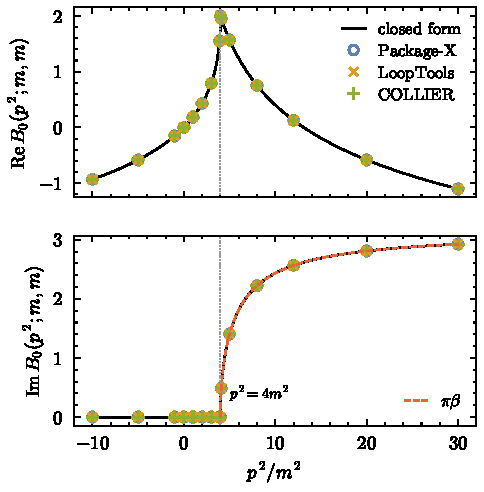
\includegraphics[width=0.6\linewidth]{../figs/b0_d4.pdf}
\caption{$B_0(p^2;m,m)$ の実部（上）と虚部（下）（$m=\mu=1$、$\Delta=0$）。実線は\ref{app:b0} の閉じた式、記号は Package-X・LoopTools・COLLIER の値、下の破線は $\pi\beta$、点線は閾値 $p^2=4m^2$ である。}
\label{fig:b0}
\end{figure}

\section{議論と今後}\label{sec:discussion}

\paragraph{決まっていないこと。}有限部分の規約（$\overline{\mathrm{MS}}$ か on-shell か）は、有限部分を比べる段階で決める必要がある。on-shell にすると、$d=4$ でも $\delta_Z$ に有限の寄与が生じる。$d=6$ の有限部分は Package-X と LoopTools で検算できないので、Feynman パラメータ積分の数値計算が唯一の独立な検算になる。2ループ用に推奨された pySecDec などが入れば、それが二つ目の検算手段になる~\cite{review}。

\paragraph{タドポールの扱い。}本ノートでは、$Y$ でタドポールを打ち消す方法をとった。これは1ループでは、FeynArts でタドポールの位相（\texttt{Tadpoles}）を除くことと同じである。2ループ以上では、ループの内側にタドポールが付いた図も $Y$ の高次の項で消えるので、同じ除き方で済むかどうかを確かめる必要がある。

\paragraph{LoopTools の $C_0$。}手順 (3) で見つかった LoopTools の $C_0$ の誤りは、コンパイラの版や最適化によらない。そのため、この Mac（Apple M3）上での LoopTools 2.16 の問題である可能性が高いが、原因は突き止めていない。当面、$C_0$ には Package-X と COLLIER を使い、LoopTools は $A_0$ と $B_0$ にだけ使う。Fortran から \texttt{C0(1D0,1D0,1D0,1D0,1D0,1D0)} を呼ぶと止まるという最小の再現例があるので、開発者に報告できる。

\paragraph{今後。}次は第~\ref{sec:plan} 節の手順 (4)、$d=6$ の1ループの検算である。FeynCalc で $D=6-2\epsilon$ として計算し、式~\eqref{eq:ct6} と式~\eqref{eq:beta6} を再現する。

\appendix

\section{Feynman 則と対称性因子の導出}\label{app:rules}

\paragraph{伝播関数。}自由部分の作用は、部分積分して $S_0=\int\dd^dx\,\tfrac12\phi(-\partial^2-m^2)\phi$ と書ける。2点関数 $\langle0|T\phi(x)\phi(y)|0\rangle$ は演算子 $(-\partial^2-m^2)$ の逆に $i$ を掛けたもので、Fourier 変換 $\phi(x)=\int\dd^dp/(2\pi)^d\,e^{-ip\cdot x}\tilde\phi(p)$ のもとで $-\partial^2\to p^2$ となる。よって運動量空間の伝播関数は $i/(p^2-m^2+i0)$ である。$+i0$ は時間順序積を与える Feynman の処方である。

\paragraph{頂点。}相互作用の部分 $\mathcal{L}_{\text{int}}=-(g\mu^\epsilon/3!)\phi^3+Y\phi$ から、頂点の因子は「$i\times$（$\mathcal{L}_{\text{int}}$ の係数）$\times$（同じ場の線の付け方の数）」で決まる。3点頂点では、区別できる3本の線を3つの $\phi$ に付ける方法が $3!$ 通りあるので、因子は $i\cdot(-g\mu^\epsilon/3!)\cdot3!=-ig\mu^\epsilon$ となる。線形項は $1$ 通りで $iY$ である。対抗項も同じ規則に従う。$\tfrac12\delta_Z\partial_\mu\phi\partial^\mu\phi-\tfrac12\delta_m\phi^2$ は2本の線の付け方が $2$ 通りあり、運動量 $p$ が流れ込むと $\partial_\mu\to\mp ip_\mu$ が2つ掛かって $\partial\phi\cdot\partial\phi\to p^2$ となる。よって因子は $i\cdot2\cdot(\tfrac12\delta_Zp^2-\tfrac12\delta_m)=i(\delta_Zp^2-\delta_m)$ である。3点の対抗項は3点頂点と同じ計算で $-i\delta_g\mu^\epsilon$ となる。

\paragraph{対称性因子。}$n$ 次の摂動項は $\frac{1}{n!}\bigl(i\int\mathcal{L}_{\text{int}}\bigr)^n$ で、各頂点に $1/3!$ が付く。Feynman 則の頂点因子にはすでに $3!$ を含めたので、図の値は「Feynman 則による値 $\times$ $N_c/(n!\,(3!)^n)$」となる。ここで $N_c$ は、その図を与える Wick の縮約の数である。この比が $1/S$（$S$ が対称性因子）に当たる。
\begin{itemize}
\item \textbf{タドポール}（$n=1$）：外の $\phi(x)$ と縮約する頂点の場の選び方が $3$ 通り、残る2つの場どうしの縮約が $1$ 通りで、$N_c=3$。よって $1/S=3/(1!\cdot3!)=1/2$。
\item \textbf{自己エネルギー}（$n=2$）：$\phi(x)$ が付く頂点の選び方が $2$、その頂点の場の選び方が $3$、$\phi(y)$ が他方の頂点のどの場に付くかが $3$、残る2本ずつの場の対の付け方が $2$ で、$N_c=2\cdot3\cdot3\cdot2=36$。よって $1/S=36/(2!\,(3!)^2)=36/72=1/2$。
\item \textbf{頂点補正の三角形}（$n=3$）：3つの外線を3つの頂点に割り当てる方法が $3!$、各頂点で外線に付ける場の選び方が $3^3$ である。各頂点に残る2本の場を、他の二つの頂点のどちらへ向けるかの選び方が $2^3$ で、それで三角形の辺の縮約は一意に決まる。よって $N_c=6\cdot27\cdot8=1296$、$1/S=1296/(3!\,(3!)^3)=1296/1296=1$。
\item \textbf{木の各チャンネル}（$n=2$、外線4本）：外線1,2が付く頂点の選び方が $2$、その頂点で1と2に付ける場の選び方が $3\cdot2$、他方の頂点で3と4に付ける場の選び方が $3\cdot2$、残る1本ずつの場の縮約が $1$ で、$N_c=2\cdot6\cdot6=72$。よって $1/S=72/(2!\,(3!)^2)=1$。
\end{itemize}

\section{次元とべき数え上げ}\label{app:counting}

\paragraph{次元。}作用 $\int\dd^Dx\,\mathcal{L}$ は無次元なので、$\mathcal{L}$ の質量次元は $D$ である。運動項 $\partial\phi\partial\phi$ から $[\phi]=(D-2)/2$ となる。$g_0\phi^3$ の次元が $D$ であることから $[g_0]=D-3(D-2)/2=3-D/2$ となり、$D=d-2\epsilon$ では $[g_0]=3-d/2+\epsilon$ である。そこで $g_0=\mu^\epsilon(g+\delta_g)Z^{-3/2}$ と書けば、$g$ の次元は $3-d/2$ になる。すなわち $d=4$ で1、$d=6$ で0である。

\paragraph{発散次数。}外線 $E$、頂点 $V$、内線 $I$、ループ $L$ の図では、ループ積分 $\dd^dk$ ごとに $d$、伝播関数ごとに $-2$ のべきが付くので、$\omega=dL-2I$ である。各頂点から3本の線が出るので $3V=E+2I$、すなわち $I=(3V-E)/2$。連結な図では $L=I-V+1$ である。これらを代入すると
\begin{equation*}
\omega=(d-2)I-dV+d=(d-2)\frac{3V-E}{2}-dV+d=d-\frac{d-2}{2}E+\frac{d-6}{2}V
\end{equation*}
となり、式~\eqref{eq:omega} を得る（線形項の頂点は $Y$ で打ち消したので数えない）。1ループ（$L=1$）では $I=V$ なので、$3V=E+2V$ から $E=V$ となり、$\omega=d-2E$ である。

\section{1ループ積分の一般式と発散部分}\label{app:integrals}

\paragraph{Feynman パラメータ。}$\mathrm{Im}\,A_j>0$ の量に対して $1/A_j=-i\int_0^\infty\dd t_j\,e^{it_jA_j}$ が成り立つ。$N$ 個の積をとり、$1=\int_0^\infty\dd\lambda\,\delta(\lambda-\sum_jt_j)$ を挿入して $t_j=\lambda x_j$ と変数変換すると、$\prod_j\dd t_j=\lambda^{N-1}\dd\lambda\prod_j\dd x_j$ かつ $\delta(\lambda-\lambda\sum x_j)=\lambda^{-1}\delta(1-\sum x_j)$ なので、
\begin{equation*}
\prod_{j=1}^N\frac{1}{A_j}=(-i)^N\int\!\dd F\int_0^\infty\dd\lambda\,\lambda^{N-1}e^{i\lambda B}
=(-i)^N\int\!\dd F\,\frac{\Gamma(N)}{(-iB)^N}=\Gamma(N)\int\!\dd F\,\frac{1}{B^N},
\qquad B=\sum_jx_jA_j .
\end{equation*}
ここで $\int\dd F\equiv\int_0^1\prod_j\dd x_j\,\delta(1-\sum_jx_j)$ であり、$\mathrm{Im}\,B>0$ のもとで $\int_0^\infty\dd\lambda\,\lambda^{N-1}e^{i\lambda B}=\Gamma(N)/(-iB)^N$ を使った。$A_j=(k+q_j)^2-m^2+i0$ は $\mathrm{Im}\,A_j>0$ を満たす。

\paragraph{運動量のずらし。}$\sum_jx_j=1$ を使うと
\begin{equation*}
B=\sum_jx_j\bigl[(k+q_j)^2-m^2\bigr]=k^2+2k\cdot Q+\sum_jx_jq_j^2-m^2=(k+Q)^2-\Delta,\qquad Q\equiv\sum_jx_jq_j,
\end{equation*}
\begin{equation*}
\Delta=m^2-\sum_jx_jq_j^2+Q^2 .
\end{equation*}
次元正則化では積分変数をずらせるので、$\ell=k+Q$ とする。

\paragraph{Wick 回転と $D$ 次元の積分。}$\Delta>0$ のとき、$\ell^0=i\ell_E^0$ と積分路を回転できる（$+i0$ の極の位置と整合する）。このとき $\dd^D\ell=i\,\dd^D\ell_E$、$\ell^2=-\ell_E^2$ なので、
\begin{equation*}
J_n(\Delta)\equiv\int\frac{\dd^D\ell}{(2\pi)^D}\frac{1}{(\ell^2-\Delta+i0)^n}=i(-1)^n\int\frac{\dd^D\ell_E}{(2\pi)^D}\frac{1}{(\ell_E^2+\Delta)^n}.
\end{equation*}
$D$ 次元の単位球面の面積は $2\pi^{D/2}/\Gamma(D/2)$ で、$t=\ell_E^2$ とすると $\ell_E^{D-1}\dd\ell_E=\tfrac12t^{D/2-1}\dd t$ なので、$\int\dd^D\ell_E\,f(\ell_E^2)=\frac{\pi^{D/2}}{\Gamma(D/2)}\int_0^\infty\dd t\,t^{D/2-1}f(t)$ となる。さらに $t=\Delta u/(1-u)$ と置くと、ベータ関数の積分
\begin{equation*}
\int_0^\infty\dd t\,\frac{t^{a-1}}{(t+\Delta)^n}=\Delta^{a-n}\int_0^1\dd u\,u^{a-1}(1-u)^{n-a-1}=\Delta^{a-n}\frac{\Gamma(a)\Gamma(n-a)}{\Gamma(n)}
\end{equation*}
を得る。$a=D/2$ とし、$\pi^{D/2}/(2\pi)^D=1/(4\pi)^{D/2}$ を使うと、
\begin{equation*}
J_n(\Delta)=\frac{i(-1)^n}{(4\pi)^{D/2}}\frac{\Gamma(n-D/2)}{\Gamma(n)}\,\Delta^{D/2-n}.
\end{equation*}

\paragraph{一般式。}以上をまとめると $I_N=\Gamma(N)\int\dd F\,J_N(\Delta)$ となり、$\Gamma(N)$ が約分されて式~\eqref{eq:IN-general} を得る。$\Delta\le0$ となる運動学では、$m^2\to m^2-i0$ による解析接続で同じ式を使う。

\paragraph{極の取り出し。}$D=d-2\epsilon$、$k=d/2-N$ とすると、$\Gamma(N-D/2)=\Gamma(-k+\epsilon)$ である。$k<0$ なら、これは $\epsilon\to0$ で有限である。$k\ge0$ の整数なら、$\Gamma(z+1)=z\Gamma(z)$ を $k+1$ 回使って
\begin{equation*}
\Gamma(-k+\epsilon)=\frac{\Gamma(1+\epsilon)}{\epsilon(\epsilon-1)(\epsilon-2)\cdots(\epsilon-k)}
=\frac{1}{\epsilon}\cdot\frac{1}{(-1)^k\,k!}\bigl(1+O(\epsilon)\bigr)
\end{equation*}
となる。残りの因子は $(4\pi)^{-D/2}=(4\pi)^{-d/2}(1+O(\epsilon))$、$\Delta^{D/2-N}=\Delta^{k}(1+O(\epsilon))$ で、有限部分にしか寄与しない。よって極の部分は式~\eqref{eq:poleN} になる。

\paragraph{$N=1,2,3$ への適用。}$N=1$（$q_1=0$）では $\int\dd F=1$、$\Delta=m^2$ である。$N=2$（$q_1=0$、$q_2=p$、$x_2=x$）では $\Delta=m^2-xp^2+x^2p^2=m^2-x(1-x)p^2$ で、$\int_0^1x(1-x)\dd x=1/6$ より $\int\dd F\,\Delta=m^2-p^2/6$ である。$N=3$ では $\int\dd F=\int_0^1\dd x\int_0^{1-x}\dd y=1/2$ である。これらを式~\eqref{eq:poleN} に入れる。
\begin{itemize}
\item $d=4$：$I_1$ は $N=1,k=1$ で $\dfrac{i(-1)^2}{(4\pi)^2\,1!\,\epsilon}m^2=\dfrac{im^2}{(4\pi)^2\epsilon}$。$I_2$ は $N=2,k=0$ で $\dfrac{i(-1)^2}{(4\pi)^2\epsilon}=\dfrac{i}{(4\pi)^2\epsilon}$。$I_3$ は $k=-1<0$ で有限。
\item $d=6$：$I_1$ は $N=1,k=2$ で $\dfrac{i(-1)^3}{(4\pi)^3\,2!\,\epsilon}m^4=-\dfrac{im^4}{2(4\pi)^3\epsilon}$。$I_2$ は $N=2,k=1$ で $\dfrac{i(-1)^3}{(4\pi)^3\epsilon}\Bigl(m^2-\dfrac{p^2}{6}\Bigr)$。$I_3$ は $N=3,k=0$ で $\dfrac{i(-1)^3}{(4\pi)^3\epsilon}\cdot\dfrac12=-\dfrac{i}{2(4\pi)^3\epsilon}$。
\end{itemize}
これが表~\ref{tab:poles} である。

\section{1PI 関数、対抗項、繰り込み群の導出}\label{app:ren}

\paragraph{1PI 関数。}Feynman 則（\ref{app:rules}）で、ループの伝播関数1本ごとに $i$ が1つ出る。それをまとめて積分 $I_N$ の外に出すと、次のようになる。タドポールは頂点1つ、伝播関数1本、対称性因子 $1/2$ なので $\frac12(-ig\mu^\epsilon)(i\,I_1)=\frac{g\mu^\epsilon}{2}I_1$。自己エネルギーは $\frac12(-ig\mu^\epsilon)^2\,i^2\,I_2=\frac12(-1)(-1)g^2\mu^{2\epsilon}I_2=\frac{g^2\mu^{2\epsilon}}{2}I_2$。三角形は $(-ig\mu^\epsilon)^3\,i^3\,I_3=\bigl((-i)\cdot i\bigr)^3g^3\mu^{3\epsilon}I_3=g^3\mu^{3\epsilon}I_3$。これに線形項 $iY$ と対抗項 $i(\delta_Zp^2-\delta_m)$、$-i\delta_g\mu^\epsilon$ を加えたものが式~\eqref{eq:V} である。$V_1=0$ から $Y=(ig\mu^\epsilon/2)I_1$。その極の部分は、$d=4$ で $Y=-gm^2/(2(4\pi)^2\epsilon)$、$d=6$ で $Y=gm^4/(4(4\pi)^3\epsilon)$ である。

\paragraph{MS の対抗項。}$\mu^{n\epsilon}=1+O(\epsilon)$ は有限部分にしか効かないので、極の条件では $1$ と置いてよい。
\begin{itemize}
\item $d=4$：$V_2$ の極は $\frac{g^2}{2}\cdot\frac{i}{(4\pi)^2\epsilon}+i(\delta_Zp^2-\delta_m)$。これが $p^2$ によらず $0$ になるには、$p^2$ の係数から $\delta_Z=0$、定数部分から $\delta_m=g^2/(2(4\pi)^2\epsilon)$。$V_3$ は有限なので $\delta_g=0$。
\item $d=6$：$V_2$ の極は $\frac{g^2}{2}\cdot\Bigl(-\frac{i}{(4\pi)^3\epsilon}\Bigr)\Bigl(m^2-\frac{p^2}{6}\Bigr)+i(\delta_Zp^2-\delta_m)$。$p^2$ の係数から $\frac{ig^2}{12(4\pi)^3\epsilon}+i\delta_Z=0$、すなわち $\delta_Z=-\frac{g^2}{12(4\pi)^3\epsilon}$。定数部分から $-\frac{ig^2m^2}{2(4\pi)^3\epsilon}-i\delta_m=0$、すなわち $\delta_m=-\frac{g^2m^2}{2(4\pi)^3\epsilon}$。$V_3$ の極は $g^3\cdot\Bigl(-\frac{i}{2(4\pi)^3\epsilon}\Bigr)-i\delta_g$ で、これを $0$ として $\delta_g=-\frac{g^3}{2(4\pi)^3\epsilon}$。
\end{itemize}
これが式~\eqref{eq:ct4} と式~\eqref{eq:ct6} である。

\paragraph{裸の量との関係。}裸のラグランジアン $\frac12(\partial\phi_0)^2-\frac12m_0^2\phi_0^2-\frac{g_0}{3!}\phi_0^3$ に $\phi_0=Z^{1/2}\phi$ を代入すると、$\frac12Z(\partial\phi)^2-\frac12Zm_0^2\phi^2-\frac{g_0Z^{3/2}}{3!}\phi^3$ となる。これを式~\eqref{eq:L} の $Y$ 以外の部分と比べると、
\begin{equation*}
Z=1+\delta_Z,\qquad Zm_0^2=m^2+\delta_m,\qquad g_0Z^{3/2}=\mu^\epsilon(g+\delta_g)
\end{equation*}
を得る。

\paragraph{$d=6$ の $\beta$ 関数。}$K\equiv(4\pi)^3$ と書く。1ループの精度で
\begin{equation*}
g_0=\mu^\epsilon(g+\delta_g)(1+\delta_Z)^{-3/2}=\mu^\epsilon\Bigl(g+\delta_g-\frac32g\,\delta_Z\Bigr)
=\mu^\epsilon\Bigl(g-\frac{g^3}{2K\epsilon}+\frac{g^3}{8K\epsilon}\Bigr)=\mu^\epsilon f(g),\qquad f(g)\equiv g-\frac{3g^3}{8K\epsilon}.
\end{equation*}
$g_0$ は $\mu$ によらないので、$0=\dd g_0/\dd\ln\mu=\mu^\epsilon\bigl[\epsilon f(g)+f'(g)\,\beta_\epsilon\bigr]$ である。ここで $\beta_\epsilon\equiv\dd g/\dd\ln\mu$（$D$ 次元での値）とした。よって
\begin{equation*}
\beta_\epsilon=-\frac{\epsilon f(g)}{f'(g)}=-\epsilon\,\frac{g-\frac{3g^3}{8K\epsilon}}{1-\frac{9g^2}{8K\epsilon}}
=-\epsilon\Bigl(g-\frac{3g^3}{8K\epsilon}\Bigr)\Bigl(1+\frac{9g^2}{8K\epsilon}\Bigr)+O(g^5)
=-\epsilon g-\frac{6g^3}{8K}+O(g^5).
\end{equation*}
$\epsilon\to0$ として $\beta(g)=-\frac{3g^3}{4K}=-\frac{3g^3}{4(4\pi)^3}$ を得る。これが式~\eqref{eq:beta6} である。$\alpha=g^2/K$ で書けば $\dd\alpha/\dd\ln\mu=2g\beta/K=-\frac32\alpha^2$ となる。

\paragraph{$d=4$ の走り。}1ループで $\delta_Z=\delta_g=0$ なので、$g_0=\mu^\epsilon g$、すなわち $\beta_\epsilon=-\epsilon g$ である。$\epsilon\to0$ で、$g$ は1ループでは走らない。質量は $Z=1$ より $m_0^2=m^2+\delta_m=m^2+\frac{g^2}{2(4\pi)^2\epsilon}$ である。$m_0^2$ が $\mu$ によらないことから
\begin{equation*}
\frac{\dd m^2}{\dd\ln\mu}=-\frac{1}{2(4\pi)^2\epsilon}\frac{\dd g^2}{\dd\ln\mu}=-\frac{1}{2(4\pi)^2\epsilon}\cdot2g\beta_\epsilon=-\frac{1}{2(4\pi)^2\epsilon}\cdot(-2\epsilon g^2)=\frac{g^2}{(4\pi)^2}
\end{equation*}
となる。これが式~\eqref{eq:mrun4} である。

\section{木レベルの振幅の導出}\label{app:tree}

$s$ チャンネルの図は、頂点2つ（$-ig$ ずつ）と、運動量 $p_1+p_2$ の伝播関数1本からなり、対称性因子は $1$ である（\ref{app:rules}）。よってその値は $(-ig)^2\,\frac{i}{s-m^2}=-\frac{ig^2}{s-m^2}$ である。$t$、$u$ チャンネルも、伝播関数の運動量が $p_1-p_3$、$p_1-p_4$ に変わるだけである。三つの和が $i\mathcal{M}$ なので、
\begin{equation*}
i\mathcal{M}=-ig^2\left[\frac{1}{s-m^2}+\frac{1}{t-m^2}+\frac{1}{u-m^2}\right]
\end{equation*}
となり、式~\eqref{eq:Mtree} を得る。木のレベルでは $\mu^\epsilon\to1$ とした。

\section{断面積の式の導出}\label{app:xsec}

\paragraph{出発点。}$2\to2$ 散乱 $p_1+p_2\to k_1+k_2$ の断面積は、流束因子と2体の位相空間を使って
\begin{equation*}
\sigma=\frac{S}{4E_1E_2|\vec v_1-\vec v_2|}\int|\mathcal{M}|^2\,\dd\Phi_2,\qquad
\dd\Phi_2=\frac{\dd^3k_1}{(2\pi)^32E_1'}\,\frac{\dd^3k_2}{(2\pi)^32E_2'}\,(2\pi)^4\delta^4(p_1+p_2-k_1-k_2)
\end{equation*}
と書ける。$E_{1,2}$ は始状態、$E'_{1,2}$ は終状態のエネルギーである。$S$ は終状態の同種粒子による因子で、終状態の角度を全立体角で積分するとき、二つの $\phi$ を二重に数えないために $S=1/2$ とする。

\paragraph{2体位相空間。}重心系では $\vec k_2=-\vec k_1$ で、$\dd^3k_2$ を $\delta^3$ で積分すると、$(2\pi)^4/(2\pi)^6=1/(4\pi^2)$ より
\begin{equation*}
\dd\Phi_2=\frac{1}{4\pi^2}\,\frac{k^2\,\dd k\,\dd\Omega}{4E_1'E_2'}\,\delta\bigl(\sqrt{s}-E_1'-E_2'\bigr),\qquad k\equiv|\vec k_1| .
\end{equation*}
$E_i'=\sqrt{k^2+m^2}$ だから、$\dd(E_1'+E_2')/\dd k=k/E_1'+k/E_2'=k(E_1'+E_2')/(E_1'E_2')$ で、根 $E_1'+E_2'=\sqrt{s}$ ではこれが $k\sqrt{s}/(E_1'E_2')$ になる。よって $\delta(\sqrt s-E_1'-E_2')=\frac{E_1'E_2'}{k_f\sqrt s}\delta(k-k_f)$ であり、
\begin{equation*}
\dd\Phi_2=\frac{1}{16\pi^2}\,\frac{k_f^2}{E_1'E_2'}\,\frac{E_1'E_2'}{k_f\sqrt s}\,\dd\Omega=\frac{k_f}{16\pi^2\sqrt s}\,\dd\Omega .
\end{equation*}

\paragraph{流束因子。}重心系では二つの速度は逆向きで、大きさは $k_i/E_1$、$k_i/E_2$ である（$k_i$ は始状態の運動量の大きさ）。よって $4E_1E_2|\vec v_1-\vec v_2|=4E_1E_2(k_i/E_1+k_i/E_2)=4k_i(E_1+E_2)=4k_i\sqrt s$ となる。

\paragraph{まとめ。}以上から
\begin{equation*}
\frac{\dd\sigma}{\dd\Omega}=S\,\frac{|\mathcal{M}|^2}{4k_i\sqrt s}\,\frac{k_f}{16\pi^2\sqrt s}=S\,\frac{|\mathcal{M}|^2}{64\pi^2s}\,\frac{k_f}{k_i}
\end{equation*}
を得る。四つの粒子の質量がすべて $m$ なら $k_f=k_i=p$、$p^2=s/4-m^2$ で $k_f/k_i=1$ となり、$S=1/2$ とともに式~\eqref{eq:sigma} になる。$|\mathcal{M}|^2$ は方位角によらないので、$\dd\Omega=2\pi\,\dd\!\cos\theta$ とした。

\paragraph{$t$ と $u$。}$\theta$ を $\vec p_1$ と $\vec k_1$ のなす角とする。$E_1=E_1'=E=\sqrt{p^2+m^2}$ なので、
\begin{equation*}
t=(p_1-k_1)^2=2m^2-2(EE-p^2\cos\theta)=2m^2-2(p^2+m^2)+2p^2\cos\theta=-2p^2(1-\cos\theta).
\end{equation*}
$u=(p_1-k_2)^2$ は $\vec k_2=-\vec k_1$ なので $\cos\theta\to-\cos\theta$ として $u=-2p^2(1+\cos\theta)$ である。確かに $s+t+u=4p^2+4m^2-4p^2=4m^2$ を満たす。

\section{$B_0$ の閉じた式と虚部の導出}\label{app:b0}

\paragraph{出発点。}式~\eqref{eq:IN-general} で $N=2$、$q_1=0$、$q_2=p$ とすると $\Delta=m^2-x(1-x)p^2$ であり、
\begin{equation*}
I_2=\frac{i\,\Gamma(\epsilon)}{(4\pi)^{2-\epsilon}}\int_0^1\dd x\,\Delta^{-\epsilon}=\frac{i}{(4\pi)^2}\,\Gamma(\epsilon)(4\pi)^{\epsilon}\int_0^1\dd x\,\Delta^{-\epsilon}
\end{equation*}
となる。$\Delta\le0$ となる運動学では $m^2\to m^2-i0$ なので、$\Delta\to\Delta-i0$ と読む。$\Gamma(\epsilon)=\Gamma(1+\epsilon)/\epsilon=1/\epsilon-\gamma_E+O(\epsilon)$（$\Gamma'(1)=-\gamma_E$）、$(4\pi)^\epsilon=1+\epsilon\ln4\pi+O(\epsilon^2)$、$\Delta^{-\epsilon}=1-\epsilon\ln\Delta+O(\epsilon^2)$ より、
\begin{equation*}
\Gamma(\epsilon)(4\pi)^\epsilon\Delta^{-\epsilon}=\frac1\epsilon-\gamma_E+\ln4\pi-\ln\Delta+O(\epsilon).
\end{equation*}
結合定数から来る $\mu^{2\epsilon}=1+2\epsilon\ln\mu+O(\epsilon^2)$ を掛けると $\ln\Delta\to\ln(\Delta/\mu^2)$ となるので、
\begin{gather*}
\mu^{2\epsilon}I_2=\frac{i}{(4\pi)^2}\Bigl[\Delta_{\mathrm{UV}}+B_0(p^2;m,m)\Bigr]+O(\epsilon),\\
\Delta_{\mathrm{UV}}\equiv\frac1\epsilon-\gamma_E+\ln4\pi,\qquad
B_0(p^2;m,m)\equiv-\int_0^1\dd x\,\ln\frac{m^2-x(1-x)p^2-i0}{\mu^2}
\end{gather*}
を得る。この $B_0$ が LoopTools の規約（$\Delta=0$）の値で、$\overline{\mathrm{MS}}$ の有限部分にあたる。$a\equiv p^2/m^2$、$D(x)\equiv1-ax(1-x)$ と置くと、$m^2>0$ より
\begin{equation*}
B_0=-\ln\frac{m^2}{\mu^2}-I(a),\qquad I(a)\equiv\int_0^1\dd x\,\ln\bigl(D(x)-i0\bigr).
\end{equation*}

\paragraph{補助積分。}実数 $c$ に対して
\begin{equation*}
\int_0^1\dd x\,\ln|x-c|=(1-c)\ln|1-c|+c\ln|c|-1
\end{equation*}
が成り立つ。実際、$x\ne c$ で $\frac{\dd}{\dd x}\bigl[(x-c)\ln|x-c|-x\bigr]=\ln|x-c|$ であり、この原始関数は $t\ln|t|\to0$（$t\to0$）より $x=c$ でも連続なので、両端の値の差が上式になる。

\paragraph{根。}$a\ne0$ のとき $D(x)=ax^2-ax+1=a(x-x_+)(x-x_-)$、$x_\pm=(1\pm\beta)/2$、$\beta\equiv\sqrt{1-4/a}$ と因数分解できる。根と係数の関係から $x_++x_-=1$、$x_+x_-=1/a$ であり、$x_+-x_-=\beta$、$1-x_\pm=x_\mp$、$2x_\pm-1=\pm\beta$ が成り立つ。$\beta$ は $a<0$ で $\beta>1$、$a>4$ で $0<\beta<1$ の実数である。

\paragraph{$a<0$。}$x_-=(1-\beta)/2<0$、$x_+>1$ なので、$[0,1]$ 上で $(x-x_+)(x-x_-)<0$ であり、$a<0$ と合わせて $D>0$ となる（$i0$ は効かない）。よって $\ln D=\ln(-a)+\ln|x-x_+|+\ln|x-x_-|$ である。補助積分と $1-x_\pm=x_\mp$ から
\begin{equation*}
\int_0^1\ln|x-x_+|\,\dd x=x_-\ln|x_-|+x_+\ln x_+-1,\qquad
\int_0^1\ln|x-x_-|\,\dd x=x_+\ln x_++x_-\ln|x_-|-1 .
\end{equation*}
また $|x_+x_-|=-1/a$ から $\ln(-a)=-\ln x_+-\ln|x_-|$ である。これらを足すと、$|x_-|=(\beta-1)/2$ を使って
\begin{equation*}
I(a)=-2+(2x_+-1)\ln x_++(2x_--1)\ln|x_-|=-2+\beta\ln\frac{x_+}{|x_-|}=-2+\beta\ln\frac{\beta+1}{\beta-1}
\end{equation*}
となり、$B_0=-\ln(m^2/\mu^2)+2+\beta\ln\dfrac{\beta-1}{\beta+1}$ を得る。

\paragraph{$a>4$。}$0<x_-<x_+<1$ で、$x_-<x<x_+$ では $D<0$ である。$D-i0$ の偏角は $-\pi$ なので、そこでは $\ln(D-i0)=\ln|D|-i\pi$ となる。$\ln|D|=\ln a+\ln|x-x_+|+\ln|x-x_-|$ に、上と同じ補助積分（今度は $x_\pm>0$）と $\ln a=-\ln x_+-\ln x_-$ を使うと、
\begin{gather*}
\mathrm{Re}\,I(a)=-2+(2x_+-1)\ln x_++(2x_--1)\ln x_-=-2+\beta\ln\frac{x_+}{x_-}=-2+\beta\ln\frac{1+\beta}{1-\beta},\\
\mathrm{Im}\,I(a)=-\pi(x_+-x_-)=-\pi\beta
\end{gather*}
となる。よって $B_0=-\ln(m^2/\mu^2)+2+\beta\ln\dfrac{1-\beta}{1+\beta}+i\pi\beta$ である。

\paragraph{$a=0$ と $a=4$。}$a=0$ では $D=1$ で $I=0$、$B_0=-\ln(m^2/\mu^2)$ である。$a=4$ では $D=(1-2x)^2\ge0$ で、$u=1-2x$ と置くと $I=2\int_0^1\ln|1-2x|\,\dd x=\int_{-1}^{1}\ln|u|\,\dd u=2\int_0^1\ln u\,\dd u=-2$ となり、$B_0=-\ln(m^2/\mu^2)+2$ である。

\paragraph{$0<a<4$。}$D>0$ で実根を持たない。部分積分すると、$D(1)=1$ より境界項が消えて
\begin{equation*}
I(a)=\bigl[x\ln D\bigr]_0^1-\int_0^1\dd x\,\frac{xD'(x)}{D(x)}=-\int_0^1\dd x\,\frac{2ax^2-ax}{D(x)}
\end{equation*}
となる（$D'(x)=2ax-a$）。分子を $2ax^2-ax=2D(x)+(ax-2)$、さらに $ax-2=\tfrac12D'(x)+\tfrac{a-4}{2}$ と分け、$\int_0^1D'/D\,\dd x=[\ln D]_0^1=0$ を使うと、
\begin{equation*}
I(a)=-2-\frac{a-4}{2}\int_0^1\frac{\dd x}{D(x)} .
\end{equation*}
$D(x)=a\bigl[(x-\tfrac12)^2+b^2\bigr]$、$b^2=(4-a)/(4a)>0$ と平方完成すると、
\begin{equation*}
\int_0^1\frac{\dd x}{D(x)}=\frac{1}{ab}\Bigl[\arctan\frac{x-1/2}{b}\Bigr]_0^1=\frac{2}{ab}\arctan\frac{1}{2b}.
\end{equation*}
$\tilde\beta\equiv\sqrt{4/a-1}$ と置くと $(4-a)/(ab)=2\tilde\beta$、$1/(2b)=1/\tilde\beta$ なので、$I(a)=-2+2\tilde\beta\arctan(1/\tilde\beta)$、すなわち $B_0=-\ln(m^2/\mu^2)+2-2\tilde\beta\arctan(1/\tilde\beta)$ である。以上の五つの場合が、\texttt{oneloop4\_numeric.py} の閉じた式である。

\paragraph{虚部と光学定理。}以上から $\mathrm{Im}\,B_0=\pi\beta\,\theta(p^2-4m^2)$ である。虚部は、二つの $\phi$ を実際に生成できる閾値 $p^2=4m^2$ から現れる。これを崩壊幅と結びつける。1PI の2点関数 $V_2$ を伝播関数 $D=i/(p^2-m^2)$ に繰り返し挿入すると、$D+DV_2D+\cdots=D/(1-V_2D)=i/(p^2-m^2-iV_2)$ となる。そこで自己エネルギーを $\Sigma\equiv iV_2$ と定義すると、完全な伝播関数は $i/(p^2-m^2-\Sigma)$ である。式~\eqref{eq:V} と上の結果から、有限部分は
\begin{equation*}
\Sigma=i\cdot\frac{g^2}{2}\,\mu^{2\epsilon}I_2=i\cdot\frac{g^2}{2}\cdot\frac{i}{(4\pi)^2}\bigl(\Delta_{\mathrm{UV}}+B_0\bigr)=-\frac{g^2}{2(4\pi)^2}\bigl(\Delta_{\mathrm{UV}}+B_0\bigr),\qquad
\mathrm{Im}\,\Sigma=-\frac{g^2\pi\beta}{2(4\pi)^2}=-\frac{g^2\beta}{32\pi}
\end{equation*}
となる。一方、質量 $M\equiv\sqrt{p^2}>2m$ の $\phi^*$ が二つの $\phi$ に崩壊する幅を求める。木の振幅の大きさは頂点 $-ig$ から $|\mathcal{M}|=g$ である。\ref{app:xsec} の2体位相空間は、$k_f=M\beta/2$ を使って $\int\dd\Phi_2=4\pi k_f/(16\pi^2M)=\beta/(8\pi)$ となる。同種粒子の因子 $1/2$ も含めて
\begin{equation*}
\Gamma(\phi^*\to\phi\phi)=\frac{1}{2M}\cdot\frac12\cdot g^2\cdot\frac{\beta}{8\pi}=\frac{g^2\beta}{32\pi M}.
\end{equation*}
よって $\mathrm{Im}\,\Sigma=-M\,\Gamma(\phi^*\to\phi\phi)$ が成り立つ。これは自己エネルギーに対する光学定理（ユニタリー性）であり、完全な伝播関数が $i/(p^2-m^2-\mathrm{Re}\,\Sigma+iM\Gamma)$ という Breit--Wigner 形になることと整合する。

\begin{thebibliography}{9}
\small
\bibitem{srednicki} M. Srednicki, \textit{Quantum Field Theory} (Cambridge University Press, 2007)。$d=6$ の $\phi^3$ 理論の繰り込み（第9--28章）。$d=6-\epsilon_{\mathrm S}$ の規約を使う。本ノートの式~\eqref{eq:ct6} との照合は、同書の値を記憶から引いたもので、式番号は未照合である。
\bibitem{peskin} M. E. Peskin, D. V. Schroeder, \textit{An Introduction to Quantum Field Theory} (Addison-Wesley, 1995)。Feynman パラメータと $D$ 次元の積分（第6章、付録A）。
\bibitem{env} ループ計算環境の構築記録（本リポジトリ \nolinkurl{environment/environment.pdf}、2026年10月9日）。
\bibitem{review} Feynman 図のループ計算支援ツールの比較レビュー（本リポジトリ \nolinkurl{loop_tools_review/loop_tools_review.pdf}）。
\end{thebibliography}

\end{document}
